\documentclass[10pt,handout]{beamer} 
\PassOptionsToPackage{most}{tcolorbox}
\usetheme{jambro}
\tcbuselibrary{listings}
\graphicspath{{./Replic/SW2001/}{./Replic/BQ1989/}{./Replic/Uhlig2005/}{./Replic/ADRR2018/}{./Replic/GK2015/}{./Replic/JT2025/}}
\usepackage{wasysym}
\hypersetup{colorlinks,citecolor=main,linkcolor=white,urlcolor=main}
\usepackage{newverbs}
\usepackage{courier} 

% MATLAB code environments (matches handbook: matlabcode, matlaboutput)
% Note: frames containing matlabcode/matlaboutput must use \begin{frame}[fragile]
%-----------------------------------------------------
\makeatletter
\newcommand*\codesize{\@setfontsize\codesize{8.0}{9.5}}
\newcommand*\codesizebox{\@setfontsize\codesizebox{7.0}{8.5}}
\makeatother
% Inline monospace highlight, imported from handbook (VAR_Handbook.tex)
\newcommand{\mc}[1]{\colorbox{script!80}{\codesize\texttt{#1}}}
\definecolor{matlabbg}{RGB}{255,248,225}
\lstdefinestyle{matlab}{
language=Matlab,
basicstyle=\codesizebox\ttfamily,
keywordstyle=\color{matlabblue},
commentstyle=\color{matlabgreen},
stringstyle=\color{matlabpurple},
numberstyle=\tiny\color{gray},
numbers=none,
breaklines=true,
breakatwhitespace=true,
showstringspaces=false,
tabsize=4,
keepspaces=true,
columns=flexible,
frame=none,
backgroundcolor=\color{matlabbg},
xleftmargin=3pt,
xrightmargin=3pt,
aboveskip=0pt,
belowskip=0pt,
deletekeywords={detc,beta,sign,NaN,type,pi},
}
\lstset{style=matlab}
\newtcblisting{matlabcode}{
listing only,
listing options={style=matlab},
colback=script,
colframe=black!50,
boxrule=0.6pt,
arc=2pt,
left=3pt, right=3pt, top=3pt, bottom=3pt,
width=0.92\textwidth,          % slightly narrower so the box looks centered in a list
before={\par\vspace{6pt}\centering},
after={\par},
breakable,
}
\newenvironment{matlaboutput}
{\par\vspace{6pt}\codesize\ttfamily\Verbatim}
{\endVerbatim\par\vspace{6pt}\normalsize}

% Note box (matches handbook notebox: note!15 background, hand font header)
%-----------------------------------------------------
\definecolor{notebg}{RGB}{225,230,240}
\DeclareRobustCommand{\hand}{%
\fontfamily{augie}\fontseries{m}\fontshape{n}\selectfont}
\newcommand{\handdotfill}{%
\leavevmode\xleaders\hbox{{\hand\small ·}\,}\hfill\kern0pt}
% #1 = title (default: Note); #2 = extra tcolorbox options (e.g. height fill)
\newtcolorbox{notebox}[2][Note]{%
enhanced,
colback=notebg,  colframe=title,  boxrule=0.5pt,
left=6pt, right=6pt, top=4pt, bottom=6pt,
before upper={%
\noindent\handdotfill\enskip{\color{title}#1}\enskip\handdotfill\par\smallskip%
\sffamily\small},
#2
}
% Bottom spacer that shifts the (valign lower=center) body up by half the title
% strip, so the body's midpoint lands on the slide centre rather than on the
% centre of the space left below the title. Constant across boxes (single-line
% \large titles). Place just before the end of the box.
\newcommand{\noteboxcenter}{\vspace*{0.9cm}}

% Authors/institutes/date/etc
%-----------------------------------------------------
\title[VAR models]{\textbf{Applications and Replications}}
\subtitle{VAR Toolbox 4.0}
\author[]{Ambrogio Cesa-Bianchi}
\date{\today}

\begin{document}

%===============================
\section{Introduction}
%===============================

\begin{frame}[plain]
\titlepage
\end{frame}

%------------------------------------------

\begin{frame}
{\textbf{Applications and replications}}
\begin{itemize}
\item Six canonical applications from the monetary macroeconomics literature, one for each identification strategy\smallskip
\begin{itemize}
\item \cite{StockWatson2001} $\longrightarrow$ Zero short-run restrictions\medskip
\item \cite{BlanchardQuah1989} $\longrightarrow$ Zero long-run restrictions\medskip
\item \cite{Uhlig2005} $\longrightarrow$ Sign restrictions\medskip
\item \cite{AntolinDiazRubioRamirez2018} $\longrightarrow$ Narrative sign restrictions\medskip
\item \cite{GertlerKaradi2015} $\longrightarrow$ External instruments\medskip
\item \cite{JordaTaylor2025} $\longrightarrow$ Local projections (LP-OLS and LP-IV)\bigskip
\end{itemize}
\item All scripts are in \texttt{Replic/} and named \texttt{GO\_<Author><Year>.m}
\end{itemize}
\end{frame}

%===============================
\section[SW (2001)]{Stock and Watson (2001, JEP)}
%===============================

\begin{frame}
\color{title}\centering{\huge \textbf{Applications and Replications}} \par\bigskip
\color{note}\centering{\Large \textbf{Stock and Watson (2001, JEP)}}
\end{frame}

%------------------------------------------

\begin{frame}
{\textbf{Stock and Watson (2001): Zero short-run restrictions}}
\begin{minipage}{0.4\textwidth}
\begin{itemize}
\item \cite{StockWatson2001}. \textquotedblleft Vector Autoregressions,\textquotedblright\ \textit{Journal of Economic Perspectives}\bigskip
\item US\ quarterly data from 1960:Q1 to 2000:Q4\bigskip
\item Three variables: inflation ($\pi_t$), unemployment ($u_t$), federal funds rate ($r_t$)
\end{itemize}
\end{minipage}
\quad
\begin{minipage}{0.55\textwidth}
\centering
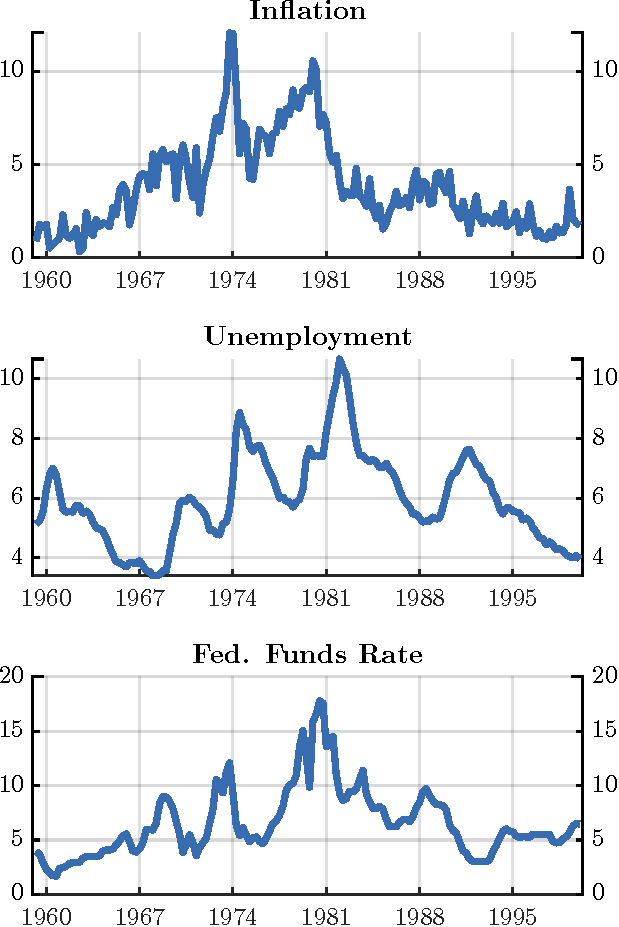
\includegraphics[width=.5\textwidth]{SW_Data.pdf}
\end{minipage}
\end{frame}

%------------------------------------------

\begin{frame}
{\textbf{What are the effects of monetary policy on output?}}
\begin{itemize}
\item \textbf{Objective} \ Infer the causal influence of monetary policy (MP) on unemployment and inflation\bigskip\pause
\item VAR with $p=4$ and a constant: inflation ($\pi_t$), unemployment ($u_t$), federal funds rate ($r_t$)\bigskip
\item \textbf{Key identifying assumptions}\smallskip
\begin{itemize}
\item MP\ ($r_{t}$) responds contemporaneously to inflation and unemployment\medskip
\item MP shocks do not affect inflation or unemployment within the quarter
\end{itemize}\pause
\end{itemize}
\begin{equation*}
\begin{bmatrix}
\pi_{t} \\ u_{t} \\ r_{t}
\end{bmatrix}
=\sum_{p=1}^4 \Phi_p x_{t-p} +\left[
\begin{array}{ccc}
b_{11} & 0 & 0 \\
b_{21} & b_{22} & 0 \\
b_{31} & b_{32} & b_{33}
\end{array}
\right]
\begin{bmatrix}
\varepsilon^{1}_{t} \\ \varepsilon^{2}_{t} \\ \varepsilon^{MonPol}_{t}
\end{bmatrix}
\end{equation*}
\end{frame}

%------------------------------------------

\begin{frame}[fragile]
{\textbf{Replicating Stock and Watson (2001) with the VAR Toolbox}}
\begin{itemize}
\item Load the data, set the lag order, and configure recursive (\texttt{'short'}) identification with bootstrap inference
\par\smallskip
\begin{matlabcode}
% Data and lag order
X = [DATA.infl, DATA.unemp, DATA.ff];
nlags = 4;  detc = 1;
% Identification setup and impulse responses with bootstrap bands
VARopt = VARoption;
VARopt.vnames    = {'Inflation','Unemployment','Fed Funds'};
VARopt.nsteps    = 24;
VARopt.snames    = {bfeps('1'), bfeps('2'), bfeps('MonPol')};
VARopt.ident     = 'short';
VARopt.inference = 1;
\end{matlabcode}
\end{itemize}
\end{frame}

%------------------------------------------

\begin{frame}[fragile]
{\textbf{Replicating Stock and Watson (2001) with the VAR Toolbox}}
\begin{itemize}
\item Estimate the VAR and plot the impulse responses with confidence bands
\par\smallskip
\begin{matlabcode}
VAR = VARmodel(X, nlags, detc, VARopt);
VARirplot(VAR.IRbar, VARopt, VAR.IRinf, VAR.IRsup);
\end{matlabcode}
\medskip
\item \textbf{Note:} the \textbf{ordering of the variables matters} --- inflation is first, unemployment second, policy rate third; monetary policy shocks cannot affect prices or output contemporaneously
\end{itemize}
\end{frame}

%------------------------------------------

\begin{frame}
{\textbf{The effect of a monetary policy shock}}
\begin{itemize}
\item Contractionary MP shock raises inflation in the short run (price puzzle) and unemployment
\end{itemize}
\begin{figure}[h]
\centering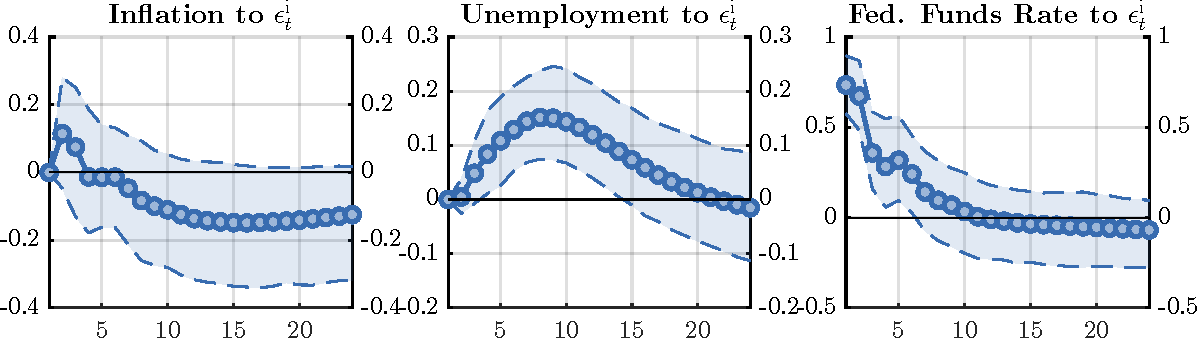
\includegraphics[width=.75\textwidth]{SW_Fig1_3.pdf}
\end{figure}
\end{frame}

%------------------------------------------

\begin{frame}
{\textbf{Shock $\varepsilon^1_t$: Supply-like pattern}}
\begin{itemize}
\item Shock $\varepsilon^1_t$ (ordered first) affects all three variables contemporaneously and behaves as a negative aggregate supply shock
\end{itemize}
\begin{figure}[h]
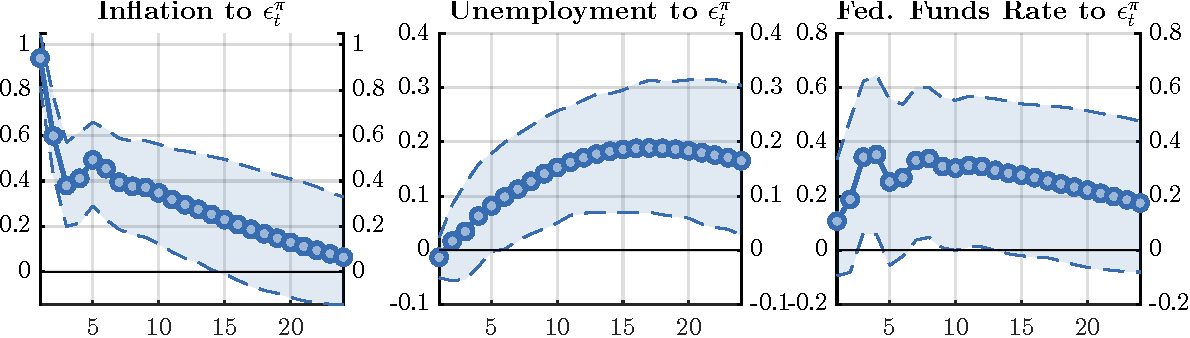
\includegraphics[width=.72\textwidth]{SW_Fig1_1.pdf}
\end{figure}
\end{frame}

%------------------------------------------

\begin{frame}
{\textbf{Shock $\varepsilon^2_t$: Demand-like pattern}}
\begin{itemize}
\item Shock $\varepsilon^2_t$ (ordered second) affects unemployment and the policy rate contemporaneously but not inflation, behaving as a negative aggregate demand shock
\end{itemize}
\begin{figure}[h]
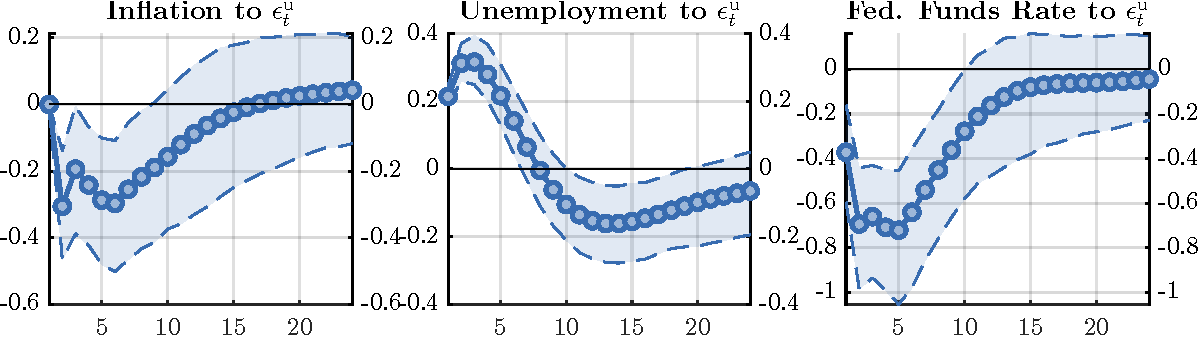
\includegraphics[width=.72\textwidth]{SW_Fig1_2.pdf}
\end{figure}
\end{frame}

%------------------------------------------

\begin{frame}
{\textbf{Forecast error variance decomposition and historical decomposition}}
\begin{figure}[h]

\includegraphics[width=.72\textwidth]{SW_VD.pdf}
\end{figure}
\end{frame}

%===============================
\section[BQ (1989)]{Blanchard and Quah (1989, AER)}
%===============================

\begin{frame}
\color{title}\centering{\huge \textbf{Applications and Replications}}\par \bigskip
\color{note}\centering{\Large \textbf{Blanchard and Quah (1989, AER)}}
\end{frame}

%------------------------------------------

\begin{frame}
{\textbf{Blanchard and Quah (1989): Zero long-run restrictions}}
\begin{minipage}{0.4\textwidth}
\begin{itemize}
\item \cite{BlanchardQuah1989}. \textquotedblleft The Dynamic Effects of Aggregate Demand and Supply Disturbances,\textquotedblright\ \emph{American Economic Review}\bigskip
\item US\ quarterly data from 1948:Q1 to 1987:Q4\bigskip
\item Two variables: GNP growth ($\Delta y_t$), unemployment ($u_t$)
\end{itemize}
\end{minipage}
\quad
\begin{minipage}{0.55\textwidth}
\centering
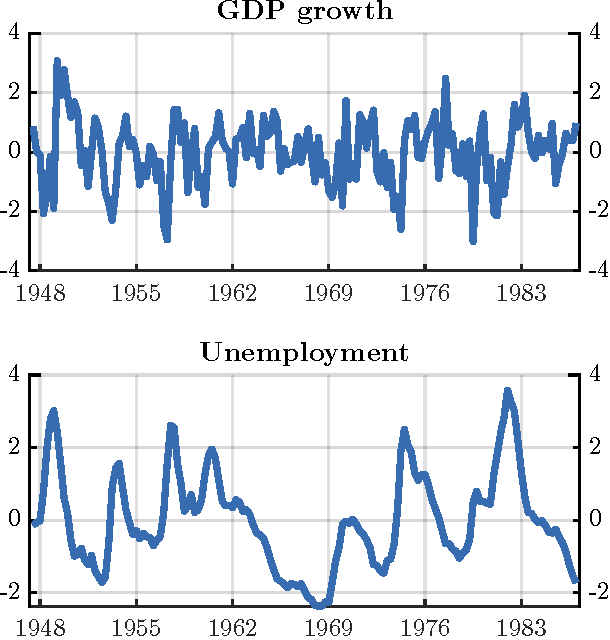
\includegraphics[width=.5\textwidth]{BQ_Data.pdf}
\end{minipage}
\end{frame}

%------------------------------------------

\begin{frame}
{\textbf{What are the effects of demand and supply shocks?}}
\begin{itemize}
\item \textbf{Objective} \ Identify the effects of demand and supply shocks on output and unemployment\bigskip\pause
\item Bivariate VAR with $p=8$: output growth ($\Delta y_t$) and unemployment ($u_t$)\bigskip
\item \textbf{Key identifying assumption} \ Demand shocks have no long-run effect on the output \textit{level}; supply shocks do\bigskip
\item The long-run impact matrix $C \equiv (I-\Phi)^{-1}B$ must be lower triangular:
\begin{equation*}
\begin{bmatrix}
\Delta y_{t,t+\infty} \\ u_{t,t+\infty}
\end{bmatrix}
=\left[
\begin{array}{cc}
c_{11} & 0 \\ c_{21} & c_{22}
\end{array}
\right]
\begin{bmatrix}
\varepsilon_t^{Supply} \\ \varepsilon_t^{Demand}
\end{bmatrix}
\end{equation*}
\end{itemize}
\end{frame}

%------------------------------------------

\begin{frame}[fragile]
{\textbf{Replicating Blanchard and Quah (1989) with the VAR Toolbox}}
\begin{itemize}
\item Load the data, set the lag order, and configure long-run (\texttt{'long'}) identification with bootstrap inference
\par\smallskip
\begin{matlabcode}
% Data and lag order
X = [DATA.y, DATA.u]; % GNP growth, unemployment
nlags = 8;  detc = 1;
% Identification setup and impulse responses with bootstrap bands
VARopt = VARoption;
VARopt.vnames    = {'GNP growth','Unemployment'};
VARopt.nsteps    = 40;
VARopt.frequency = 'q';
VARopt.snames    = {bfeps('Supply'), bfeps('Demand')};
VARopt.ident     = 'long';
VARopt.inference = 1;
\end{matlabcode}
\end{itemize}
\end{frame}

%------------------------------------------

\begin{frame}[fragile]
{\textbf{Replicating Blanchard and Quah (1989) with the VAR Toolbox}}
\begin{itemize}
\item Estimate the VAR and plot the impulse responses
\par\smallskip
\begin{matlabcode}
VAR = VARmodel(X, nlags, detc, VARopt);
VARirplot(VAR.IRbar, VARopt, VAR.IRinf, VAR.IRsup);
\end{matlabcode}
\medskip
\item \textbf{Note:} output growth is ordered first; the zero in the upper-right of $C$ imposes long-run neutrality of demand shocks on output
\end{itemize}
\end{frame}

%------------------------------------------

\begin{frame}
{\textbf{Aggregate supply shock}}
\begin{itemize}
\item Supply shock permanently raises output
\end{itemize}
\begin{figure}[h]
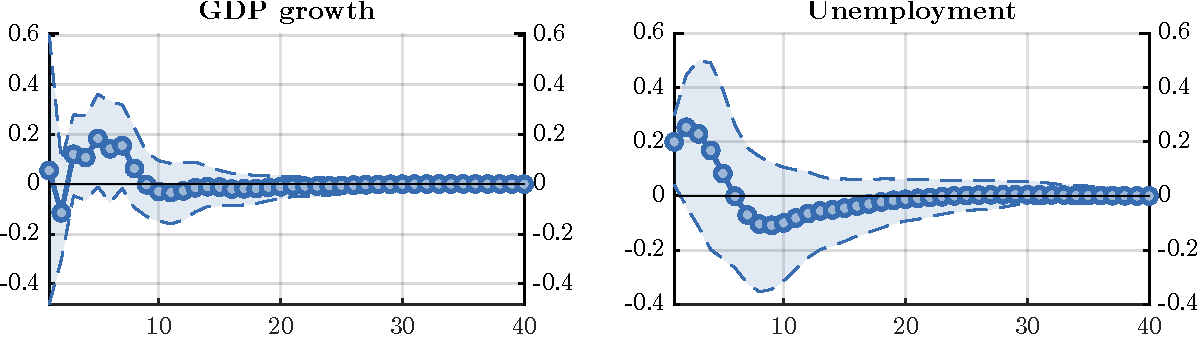
\includegraphics[width=.8\textwidth]{BQ_1.pdf}
\end{figure}
\end{frame}

%------------------------------------------

\begin{frame}
{\textbf{Aggregate demand shock}}
\begin{itemize}
\item Demand shock has a hump-shaped effect on output and unemployment, with no long-run effect on output level --- as imposed by construction
\end{itemize}
\begin{figure}[h]
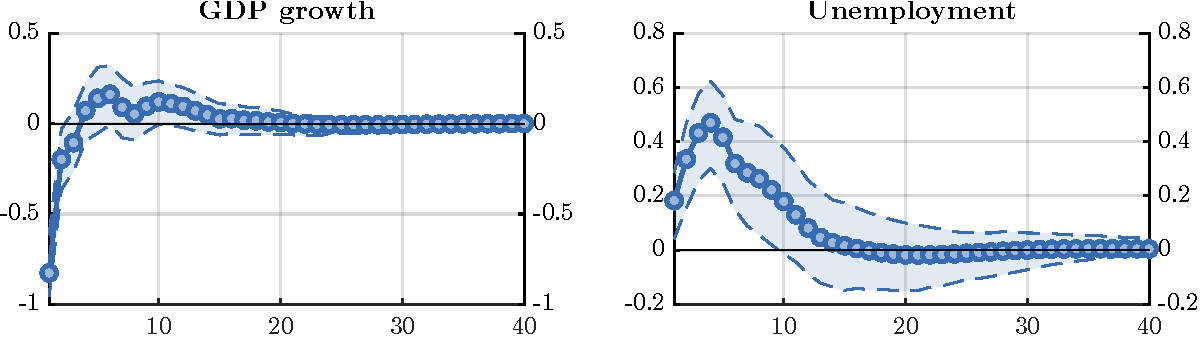
\includegraphics[width=.8\textwidth]{BQ_2.pdf}
\end{figure}
\end{frame}

%------------------------------------------

\begin{frame}
{\textbf{Long-run output level responses (Figures 1 and 2 from BQ)}}
\begin{itemize}
\item Cumulative sum of output growth responses (output level); demand shock converges to zero by construction
\end{itemize}
\begin{figure}[h]
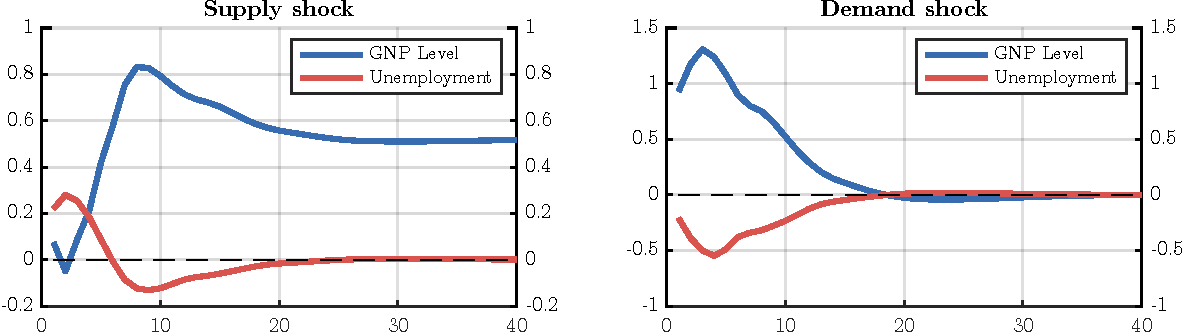
\includegraphics[width=.8\textwidth]{BQ_Fig1Fig2.pdf}
\end{figure}
\end{frame}

%===============================
\section[Uhlig (2005)]{Uhlig (2005, JME)}
%===============================

\begin{frame}
\color{title}\centering{\huge \textbf{Applications and Replications}}\par\bigskip
\color{note}\centering{\Large \textbf{Uhlig (2005, JME)}}
\end{frame}

%------------------------------------------

\begin{frame}
{\textbf{Uhlig (2005): Sign restrictions}}
\begin{minipage}{0.4\textwidth}
\begin{itemize}
\item \cite{Uhlig2005}. \textquotedblleft What are the effects of monetary policy on output?\textquotedblright\ \emph{Journal of Monetary Economics}\bigskip
\item US\ monthly data from 1965:M1 to 2003:M12
\end{itemize}
\end{minipage}
\quad
\begin{minipage}{0.55\textwidth}
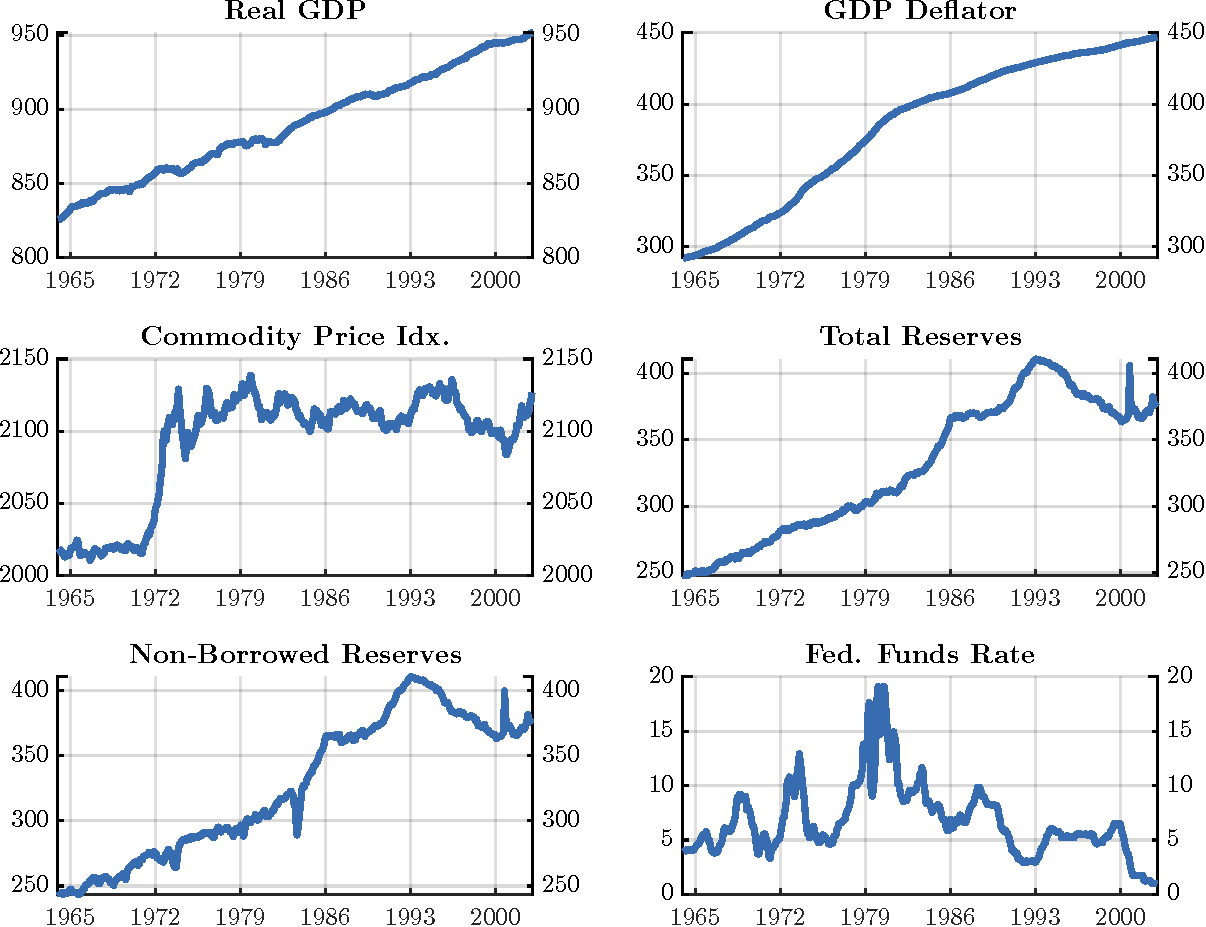
\includegraphics[width=\textwidth]{Uhlig_Data.pdf}
\end{minipage}
\end{frame}

%------------------------------------------

\begin{frame}
{\textbf{What are the effects of monetary policy on output?}}
\begin{itemize}
\item \textbf{Objective} \ Infer the causal effect of monetary policy on real GDP with minimal identifying restrictions\bigskip\pause
\item Six-variable VAR with $p=12$: real GDP, GDP deflator, commodity prices, total reserves, non-borrowed reserves, federal funds rate\bigskip
\item \textbf{Key restrictions} \ A contractionary MP shock should (for $h = 0, \ldots, 5$)\smallskip
\begin{itemize}
\item Raise the federal funds rate\medskip
\item Lower prices and non-borrowed reserves\medskip
\item Leave real GDP unrestricted (that is the object of interest!)
\end{itemize}
\end{itemize}
\end{frame}

%------------------------------------------

\begin{frame}[fragile]
{\textbf{Replicating Uhlig (2005) with the VAR Toolbox}}
\begin{itemize}
\item Set up the six-variable VAR, the number of rotation draws, and the sign-restriction horizon (\texttt{sr\_hor})
\par\smallskip
\begin{matlabcode}
% Data and lag order
X = [DATA.y, DATA.pi, DATA.comm, DATA.res, DATA.nbres, DATA.ff];
nlags = 12;  detc = 1;
% Identification setup and impulse responses
VARopt = VARoption;
VARopt.ndraws    = 500;
VARopt.sr_hor    = 6;
VARopt.inference = 1;
VARopt.nsteps    = 60;
VARopt.frequency = 'm';
VARopt.pctg      = 68;
VARopt.snames    = {bfeps('MonPol')};
\end{matlabcode}
\end{itemize}
\end{frame}

%------------------------------------------

\begin{frame}[fragile]
{\textbf{Replicating Uhlig (2005) with the VAR Toolbox}}
\begin{itemize}
\item Encode the sign restrictions in matrix $R$ (column~1 is the MP shock; rows are variables) and select \texttt{'sign'} identification
\par\smallskip
\begin{matlabcode}
% R: 1 = positive, -1 = negative, 0 = unrestricted
R = [ 0, 0, 0, 0, 0, 0;   % Real GDP (unrestricted)
     -1, 0, 0, 0, 0, 0;   % GDP Deflator (negative)
     -1, 0, 0, 0, 0, 0;   % Commodity Prices (negative)
      0, 0, 0, 0, 0, 0;   % Total Reserves (unrestricted)
     -1, 0, 0, 0, 0, 0;   % NonBorr. Reserves (negative)
      1, 0, 0, 0, 0, 0];  % Fed Funds (positive)
% Identify with sign restrictions
VARopt.ident = 'sign';
VARopt.R = R;
\end{matlabcode}
\end{itemize}
\end{frame}

%------------------------------------------

\begin{frame}[fragile]
{\textbf{Replicating Uhlig (2005) with the VAR Toolbox}}
\begin{itemize}
\item Estimate and plot; for set-identified (sign-restricted) schemes the central tendency is the median (\texttt{IRmed})
\par\smallskip
\begin{matlabcode}
VAR_sr = VARmodel(X, nlags, detc, VARopt);
VARirplot(VAR_sr.IRmed, VARopt, VAR_sr.IRinf, VAR_sr.IRsup);
\end{matlabcode}
\end{itemize}
\end{frame}

%------------------------------------------

\begin{frame}
{\textbf{Sign restriction search: First accepted rotation}}
\begin{itemize}
\item Draw random orthonormal matrices $Q$ until one $\tilde{B}=PQ$ satisfies restrictions...
\end{itemize}
\begin{figure}[h]
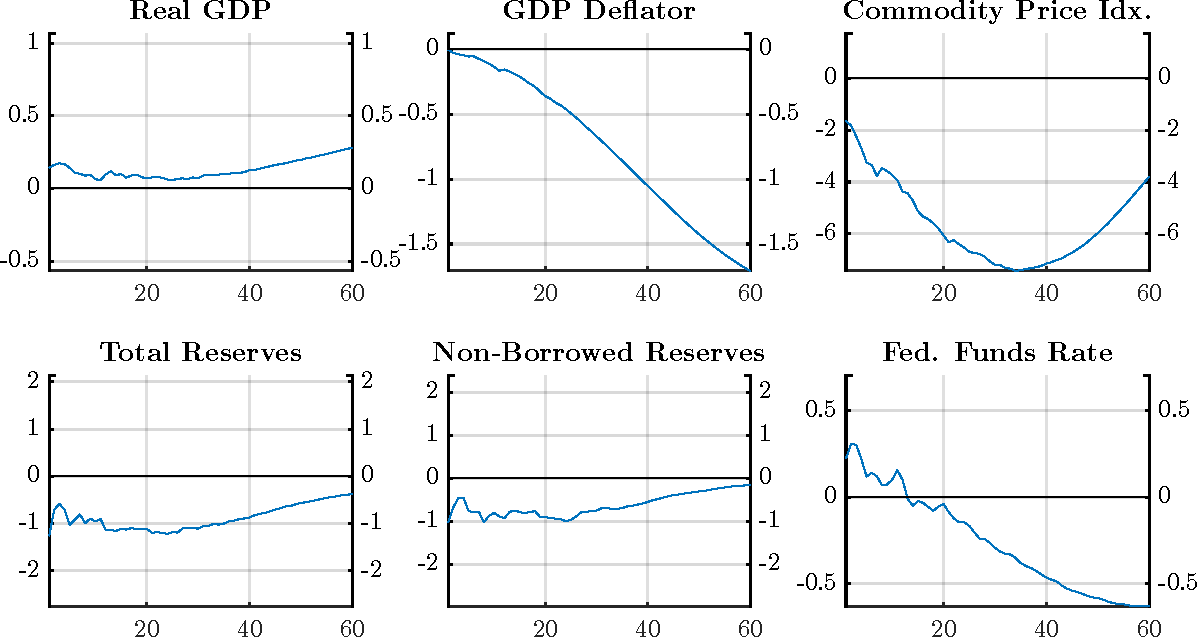
\includegraphics[width=.7\textwidth]{Uhlig_1rot_Slides.pdf}
\end{figure}
\end{frame}

%------------------------------------------

\begin{frame}
{\textbf{Sign restriction search: Two accepted rotations}}
\begin{itemize}
\item Draw another $Q$, check restrictions again... the second accepted $\tilde{B}$ is a different candidate
\end{itemize}
\begin{figure}[h]
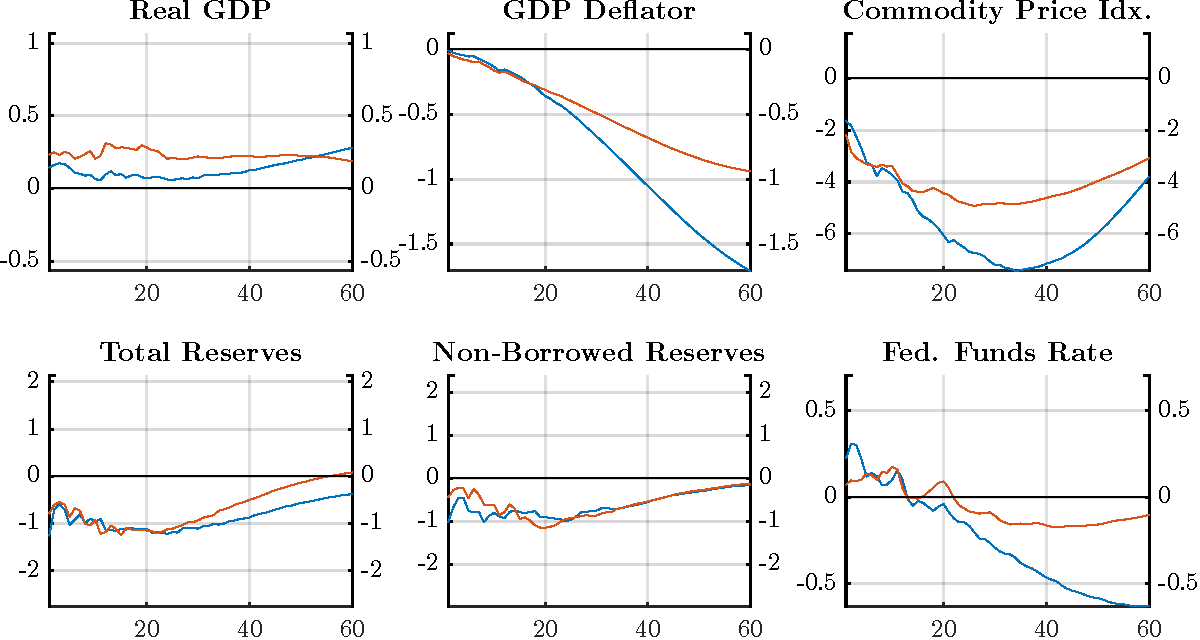
\includegraphics[width=.7\textwidth]{Uhlig_2rot_Slides.pdf}
\end{figure}
\end{frame}

%------------------------------------------

\begin{frame}
{\textbf{Sign restriction search: After many draws}}
\begin{itemize}
\item After $N$ accepted rotations, the swathe of impulse responses spans the identified set
\end{itemize}
\begin{figure}[h]
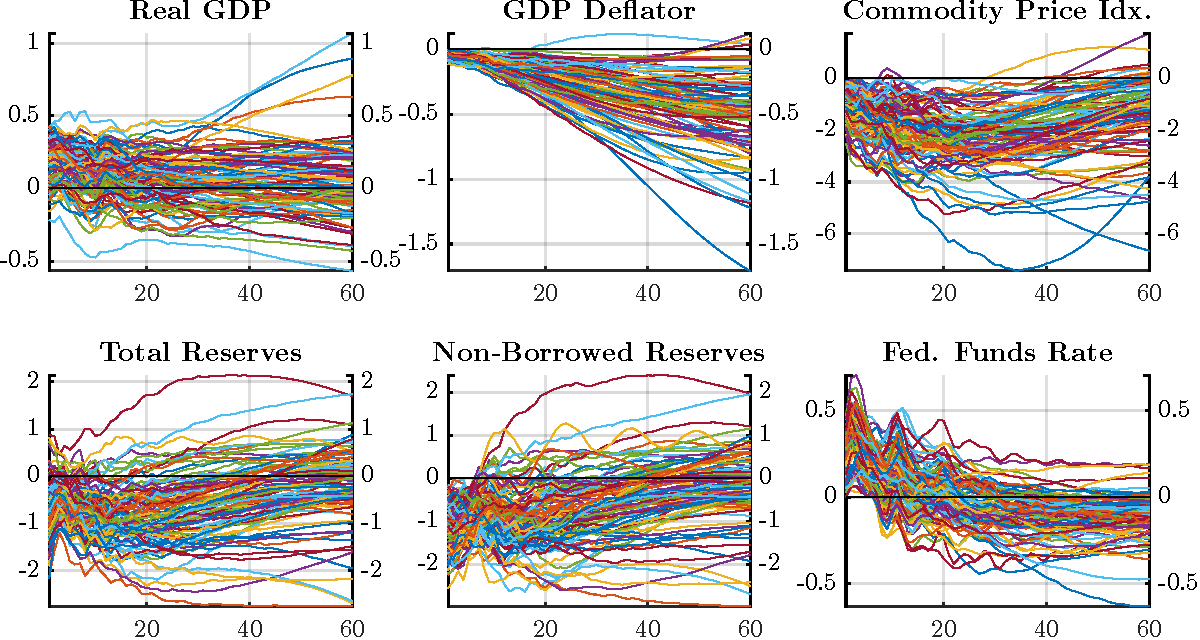
\includegraphics[width=.7\textwidth]{Uhlig_500rot_Slides.pdf}
\end{figure}
\end{frame}

%------------------------------------------

\begin{frame}
{\textbf{What are the effects of monetary policy on output?}}
\begin{itemize}
\item Output response is ambiguous $\Longrightarrow$ long-run monetary neutrality is not rejected
\end{itemize}
\begin{figure}[h]
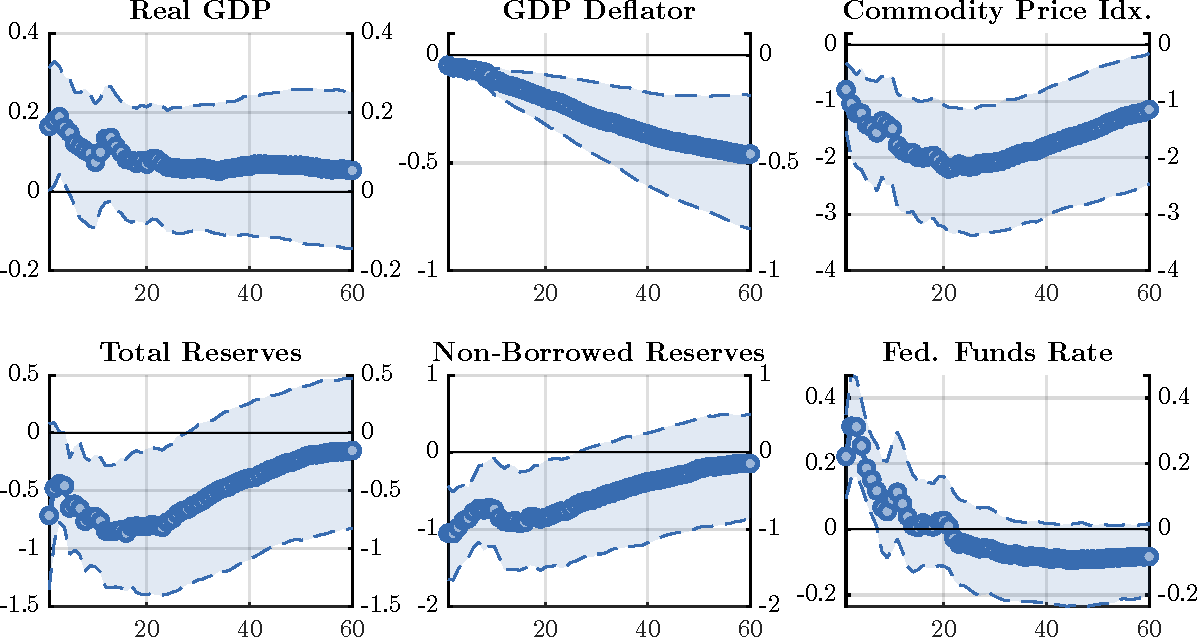
\includegraphics[width=.7\textwidth]{Uhlig_Slides.pdf}
\end{figure}
\end{frame}

%===============================
\section[ADRR (2018)]{Antol\'in-D\'iaz and Rubio-Ram\'irez (2018, AER)}
%===============================

\begin{frame}
\color{title}\centering{\huge \textbf{Applications and Replications}}\par\bigskip
\color{note}\centering{\Large \textbf{Antol\'in-D\'iaz and Rubio-Ram\'irez (2018, AER)}}
\end{frame}

%------------------------------------------

\begin{frame}
{\textbf{ADRR (2018): Narrative sign restrictions}}
\begin{minipage}{0.4\textwidth}
\begin{itemize}
\item \cite{AntolinDiazRubioRamirez2018}. \textquotedblleft Narrative Sign Restrictions for SVARs,\textquotedblright\ \textit{American Economic Review}\bigskip
\item Same six-variable VAR as Uhlig (2005)\bigskip
\item Extended sample: 1965:M1 to 2007:M11; estimated without a constant
\end{itemize}
\end{minipage}
\quad
\begin{minipage}{0.55\textwidth}
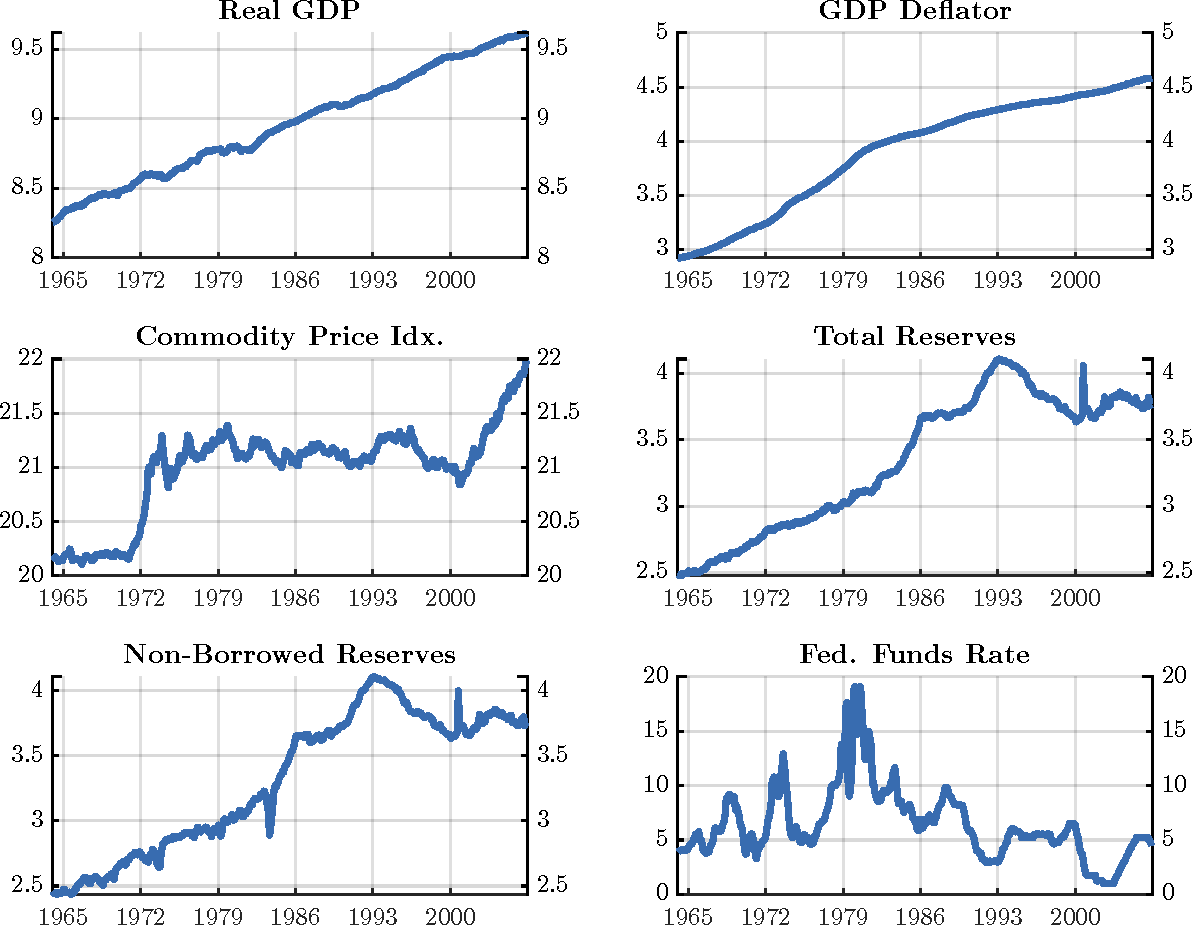
\includegraphics[width=\textwidth]{ADRR_Data.pdf}
\end{minipage}
\end{frame}

%------------------------------------------

\begin{frame}
{\textbf{Narrative episode: October 1979}}
\begin{itemize}
\item The Volcker disinflation announcement provides two pieces of narrative evidence about 1979:M10\bigskip\pause
\item \underline{\textbf{Type 1 (sign):}} \ Historical records unambiguously place the monetary policy shock in positive territory that month
\begin{equation*}
\varepsilon_{1979:M10}^{MonPol} > 0
\end{equation*}\medskip\pause
\item \underline{\textbf{Type 2 (dominance):}} \ No comparably large competing shock was operating simultaneously $\Rightarrow$ monetary policy was the dominant driver of the unexpected movement in the federal funds rate
\begin{equation*}
\bigl|b_{6m}\,\varepsilon_{1979:M10}^{MonPol}\bigr| > \sum_{k\neq m}\bigl|b_{6k}\,\varepsilon_{k,1979:M10}\bigr|
\end{equation*}
\end{itemize}
\end{frame}

%------------------------------------------

\begin{frame}[fragile]
{\textbf{Replicating ADRR (2018) with the VAR Toolbox}}
\begin{itemize}
\item Set up the VAR (no constant: \texttt{detc = 0}, data demeaned) and the sign-restriction matrix \texttt{R.sign}
\par\smallskip
\begin{matlabcode}
% Data and lag order
X = [DATA.y, DATA.pi, DATA.comm, DATA.res, DATA.nbres, DATA.ff];
nlags = 12;  detc = 0;
% Identification setup and impulse responses
VARopt = VARoption;
VARopt.nsteps = 60;
VARopt.sr_hor = 6;
VARopt.snames = {bfeps('MonPol')};
VARopt.dates  = dates;
% Sign restrictions matrix (column 1: MP shock)
R.sign = [ 0, 0, 0, 0, 0, 0;
          -1, 0, 0, 0, 0, 0;
          -1, 0, 0, 0, 0, 0;
           0, 0, 0, 0, 0, 0;
          -1, 0, 0, 0, 0, 0;
           1, 0, 0, 0, 0, 0];
\end{matlabcode}
\end{itemize}
\end{frame}

%------------------------------------------

\begin{frame}[fragile]
{\textbf{Replicating ADRR (2018) with the VAR Toolbox}}
\begin{itemize}
\item Add the two narrative restrictions targeted at October~1979 (the Volcker reform)
\par\smallskip
\begin{matlabcode}
% Type 1: MP shock positive at October 1979
R.narr_sign.shock  = 1;
R.narr_sign.period = '1979m10';
R.narr_sign.sign   = 1;
% Type 2: MP shock dominant for ff at October 1979
R.narr_dom.shock  = 1;
R.narr_dom.period = '1979m10';
R.narr_dom.var    = 6;
\end{matlabcode}
\end{itemize}
\end{frame}

%------------------------------------------

\begin{frame}[fragile]
{\textbf{Replicating ADRR (2018) with the VAR Toolbox}}
\begin{itemize}
\item Combine sign and narrative restrictions, estimate, and plot
\par\smallskip
\begin{matlabcode}
% Identify with sign + narrative restrictions
VARopt.ident = 'sign';
VARopt.R = R;
VAR_nsr = VARmodel(X, nlags, detc, VARopt);
VARirplot(VAR_nsr.IRmed, VARopt, VAR_nsr.IRinf, VAR_nsr.IRsup);
\end{matlabcode}
\end{itemize}
\end{frame}

%------------------------------------------

\begin{frame}
{\textbf{Narrative restrictions tighten the identified set}}
\begin{itemize}
\item Adding the October 1979 restrictions substantially narrows credible bands and shifts the central estimate (red) relative to sign restrictions alone (blue)
\end{itemize}
\begin{figure}[h]
\centering\includegraphics[width=.7\textwidth]{ADRR_Fig6_slides.pdf}
\end{figure}
\end{frame}

%------------------------------------------

\begin{frame}
{\textbf{Distribution of the MP shock at the narrative episode}}
\begin{itemize}
\item Distribution of $\varepsilon^{MonPol}_{1979:M10}$ across accepted draws. Sign restrictions alone (blue) leave a wide distribution; the dominance restriction (red) concentrates mass on large positive values
\end{itemize}
\begin{figure}[h]
\centering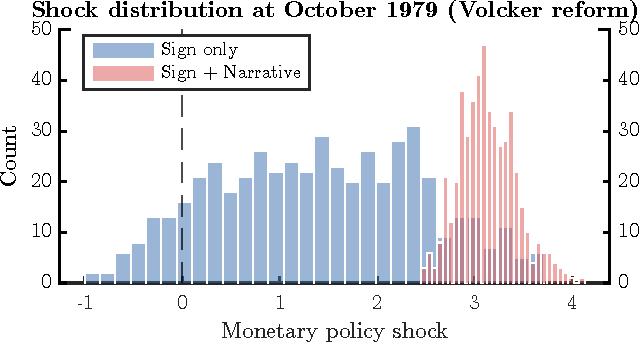
\includegraphics[width=.55\textwidth]{ADRR_Fig5.pdf}
\end{figure}
\end{frame}

%===============================
\section[GK (2015)]{Gertler and Karadi (2015, AEJ:M)}
%===============================

\begin{frame}
\color{title}\centering{\huge \textbf{Applications and Replications}}\par\bigskip
\color{note}\centering{\Large \textbf{Gertler and Karadi (2015, AEJ:M)}}
\end{frame}

%------------------------------------------

\begin{frame}
{\textbf{Gertler and Karadi (2015): External instruments}}
\begin{minipage}{0.4\textwidth}
\begin{itemize}
\item \cite{GertlerKaradi2015}. \textquotedblleft Monetary Policy Surprises, Credit Costs, and Economic Activity,\textquotedblright\ \emph{American Economic Journal: Macroeconomics}\bigskip
\item US\ monthly data from 1979:M7 to 2012:M6
\end{itemize}
\end{minipage}
\quad
\begin{minipage}{0.55\textwidth}
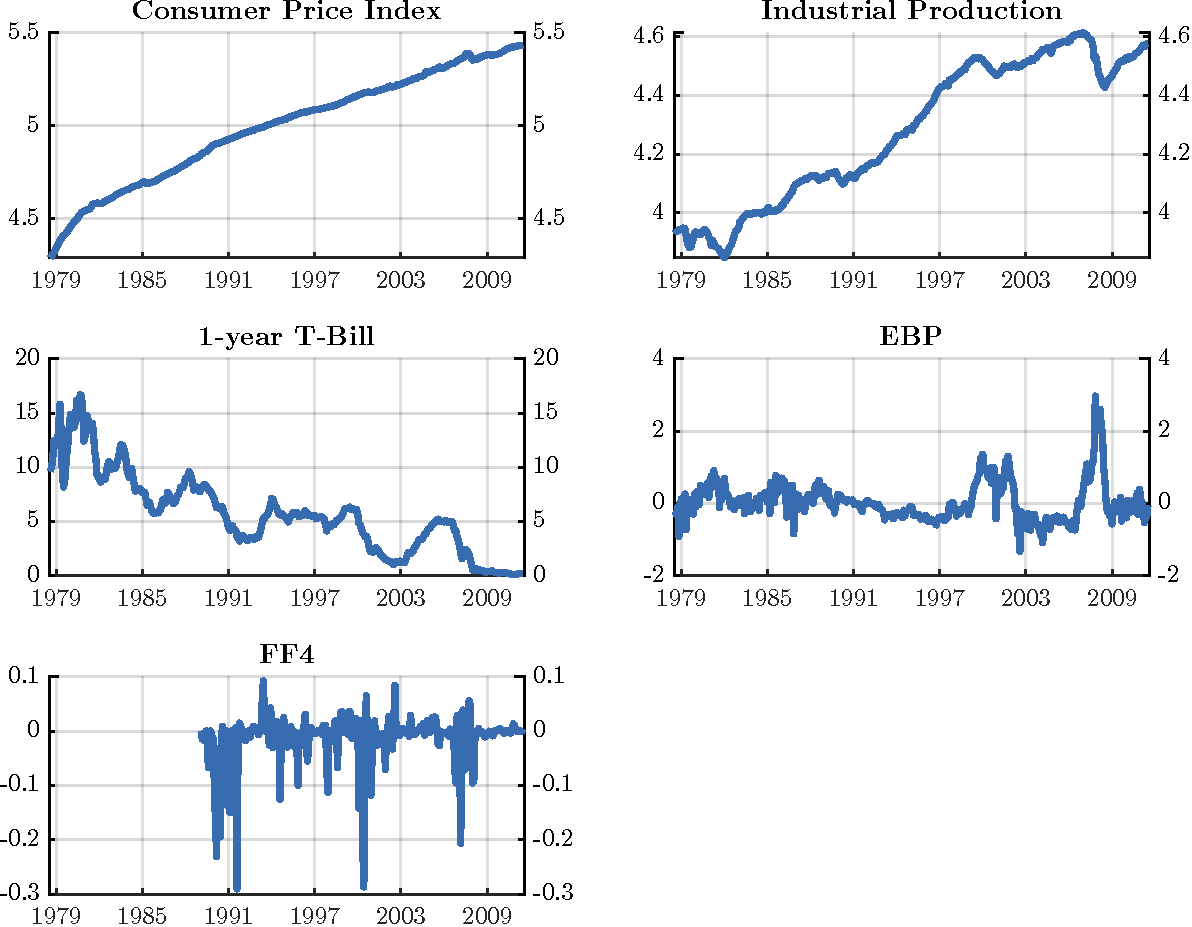
\includegraphics[width=\textwidth]{GK_Data.pdf}
\end{minipage}
\end{frame}

%------------------------------------------

\begin{frame}
{\textbf{What are the effects of monetary policy on credit markets?}}
\begin{itemize}
\item \textbf{Objective} \ Identify the credit channel of monetary transmission\bigskip\pause
\item Four-variable VAR with $p=12$: 1-year T-bill rate, CPI, industrial production, excess bond premium (EBP)\bigskip
\item \textbf{Key identifying element} \ Instrument $z_t$ constructed from high-frequency movements in federal funds futures prices around FOMC announcements:
\begin{equation*}
z_t = -(P_{t,\tau+20} - P_{t,\tau-10})
\end{equation*}
\item \textbf{1-year T-bill rate ordered first} (required by the IV implementation, which instruments the first equation's residuals)
\end{itemize}
\end{frame}

%------------------------------------------

\begin{frame}[fragile]
{\textbf{Replicating Gertler and Karadi (2015) with the VAR Toolbox}}
\begin{itemize}
\item Load the data and the FF4 futures-surprise instrument; select the wild bootstrap for heteroskedasticity-robust bands
\par\smallskip
\begin{matlabcode}
% Data, instrument, and lag order
X  = [DATA.gs1, DATA.logcpi, DATA.logip, DATA.ebp];
IV = DATA.ff4_tc;  % FF4 futures surprise
nlags = 12;  detc = 1;
% Options
VARopt = VARoption;
VARopt.nsteps    = 48;
VARopt.frequency = 'm';
VARopt.method    = 'wild';
VARopt.ndraws    = 500;
VARopt.inference = 1;
VARopt.pick      = 1;
\end{matlabcode}
\end{itemize}
\end{frame}

%------------------------------------------

\begin{frame}[fragile]
{\textbf{Replicating Gertler and Karadi (2015) with the VAR Toolbox}}
\begin{itemize}
\item Identify the same VAR two ways --- recursive (Cholesky) ordering and external instrument (proxy SVAR) --- to compare them
\par\smallskip
\begin{matlabcode}
% (1) Recursive (Cholesky) identification: policy rate ordered first
VARopt.ident     = 'short';
VAR_chol = VARmodel(X, nlags, detc, VARopt);
% (2) External-instrument identification (proxy SVAR)
VARopt.ident     = 'iv';
VARopt.IV        = IV;
VAR_iv   = VARmodel(X, nlags, detc, VARopt);
\end{matlabcode}
\end{itemize}
\end{frame}

%------------------------------------------

\begin{frame}[fragile]
{\textbf{Instrument relevance: First-stage F-statistic}}
\begin{itemize}
\item A weak instrument biases IV estimates regardless of exogeneity. Rule of thumb \cite{StockYogo2002}: $F > 10$\bigskip
\item The first-stage regression results are stored in \colorbox{script!80}{\small\texttt{VAR\_iv.FirstStage}}; the F-statistic is at \colorbox{script!80}{\small\texttt{VAR\_iv.FirstStage.F}}
\par\smallskip
\begin{matlabcode}
% Full first-stage output and the F-statistic
disp(VAR_iv.FirstStage)
F_stat = VAR_iv.FirstStage.F;
\end{matlabcode}
\medskip
\item \textbf{Key fields:} \colorbox{script!80}{\small\texttt{.F}} (F-statistic), \colorbox{script!80}{\small\texttt{.beta}} (first-stage slope $\hat{\alpha}$), \colorbox{script!80}{\small\texttt{.tstat}}, \colorbox{script!80}{\small\texttt{.rsqr}} (first-stage $R^2$)
\end{itemize}
\end{frame}

%------------------------------------------

\begin{frame}
{\textbf{Impulse response functions: Impact effect}}
\begin{itemize}
\item The impact effect ($b$ column) is recovered via the first- and second-stage IV regressions
\end{itemize}
\begin{figure}[h]
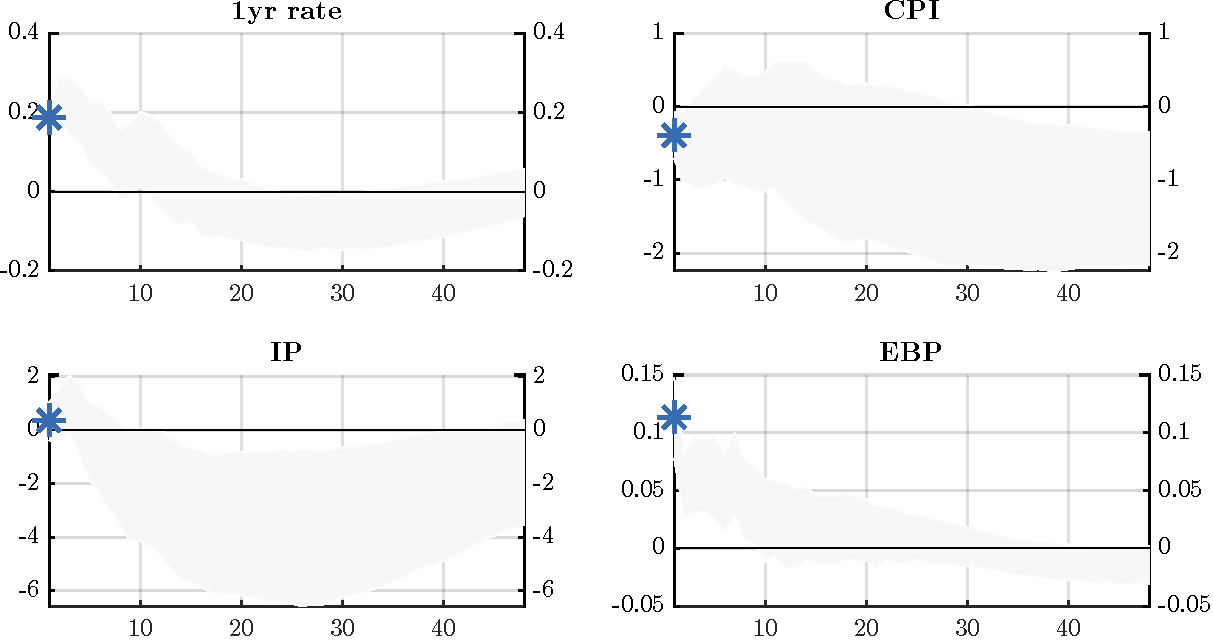
\includegraphics[width=.7\textwidth]{GK_alt_Slides.pdf}
\end{figure}
\end{frame}

%------------------------------------------

\begin{frame}
{\textbf{Impulse response functions: Dynamic effect}}
\begin{itemize}
\item Contractionary MP shock raises 1-year rate and EBP, lowers industrial production and CPI
\end{itemize}
\begin{figure}[h]
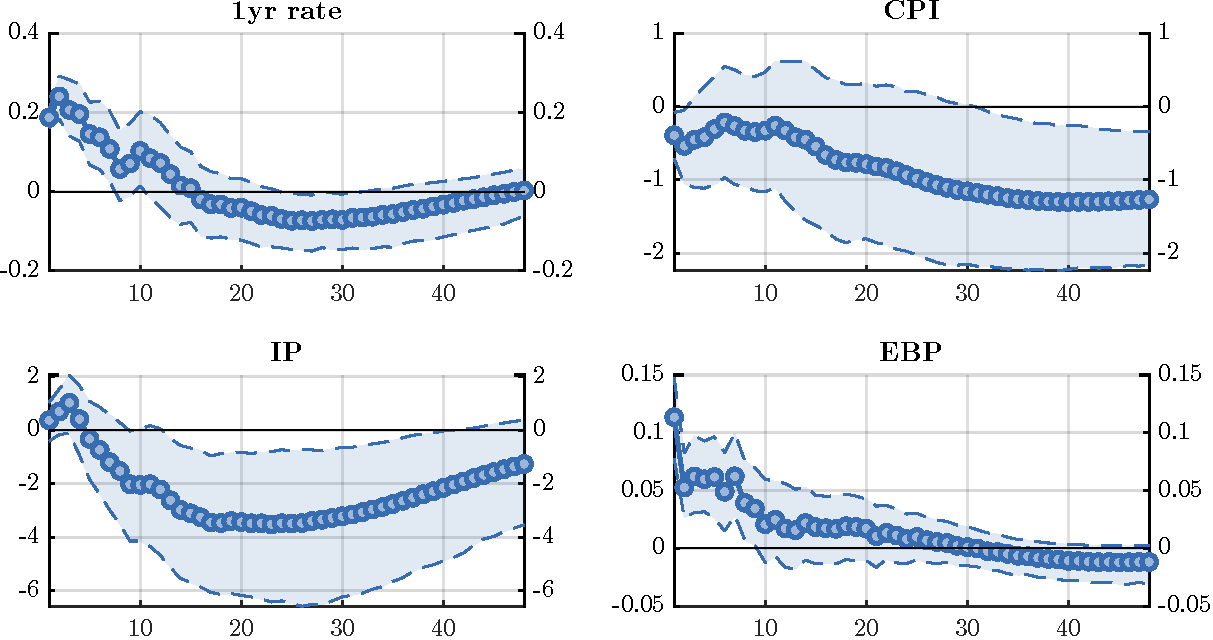
\includegraphics[width=.7\textwidth]{GK_Slides.pdf}
\end{figure}
\end{frame}

%===============================
\section[JT (2025)]{Jord\`a and Taylor (2025)}
%===============================

\begin{frame}
\color{title}\centering{\huge \textbf{Applications and Replications}}\par\bigskip
\color{note}\centering{\Large \textbf{Jord\`a and Taylor (2025)}}
\end{frame}

%------------------------------------------

\begin{frame}
{\textbf{Jord\`a and Taylor (2025): Local projections}}
\begin{itemize}
\item \cite{JordaTaylor2025}. \textquotedblleft Local Projections,\textquotedblright\ \textit{Journal of Economic Literature}\bigskip
\item \textbf{Objective} \ Illustrate LP-OLS and LP-IV on two canonical monetary applications\bigskip
\begin{itemize}
\item \textbf{Example 5 (LP-OLS):} Response of log CPI to a Romer-Romer narrative shock. Quarterly US data from 1985:Q1 to 2007:Q4. Horizon: 18 quarters\medskip
\item \textbf{Example 6 (LP-IV):} Response of unemployment to a federal funds rate shock, instrumented by the Romer-Romer (RRCG) narrative shock. Monthly US data from 1985:M1 to 2000:M1. Horizon: 49 months
\end{itemize}
\end{itemize}
\end{frame}

%------------------------------------------

\begin{frame}
{\textbf{Example 5 (LP-OLS): Data}}
\begin{minipage}{0.4\textwidth}
\begin{itemize}
\item Quarterly US data from 1985:Q1 to 2007:Q4\bigskip
\item Variables: log CPI ($\times 100$), Romer-Romer shock, log GDP growth, change in short-term interest rate\bigskip
\item CPI growth rate excluded (outcome is CPI level in long-difference form)
\end{itemize}
\end{minipage}
\quad
\begin{minipage}{0.55\textwidth}
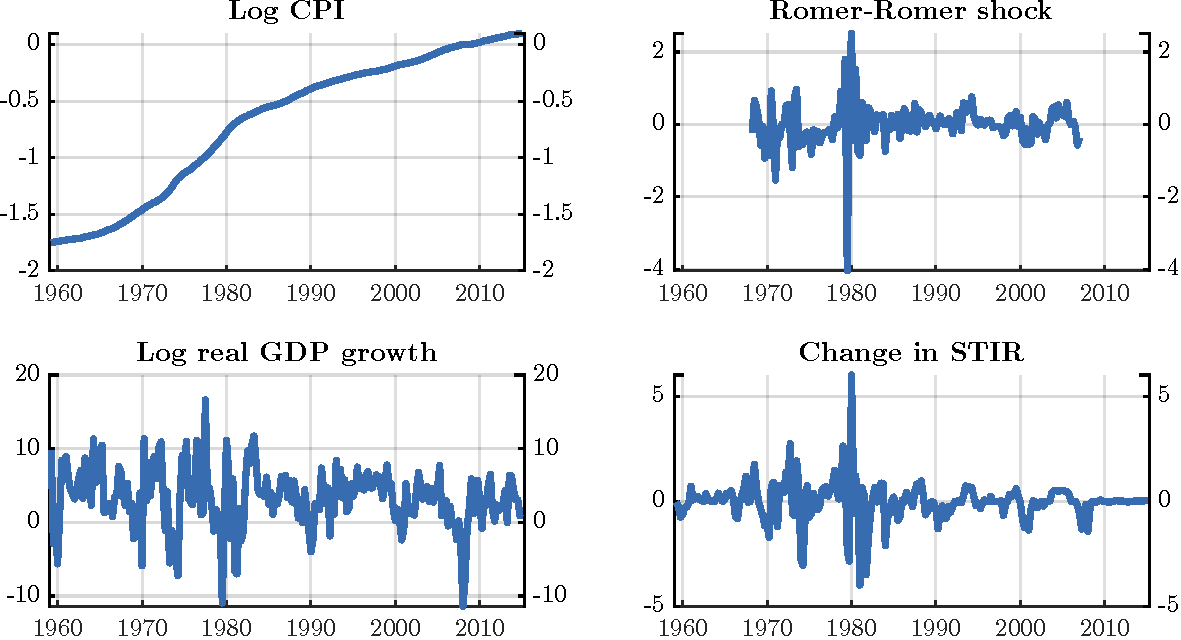
\includegraphics[width=\textwidth]{JT_Data_OLS.pdf}
\end{minipage}
\end{frame}

%------------------------------------------

\begin{frame}
{\textbf{Example 6 (LP-IV): Data}}
\begin{minipage}{0.4\textwidth}
\begin{itemize}
\item Monthly US data from 1985:M1 to 2000:M1\bigskip
\item Variables: unemployment rate (outcome), inflation, federal funds rate (endogenous treatment), RRCG narrative shock (instrument)\bigskip
\item Outcome: long-difference $\text{urate}_{t+h} - \text{urate}_{t-1}$
\end{itemize}
\end{minipage}
\quad
\begin{minipage}{0.55\textwidth}
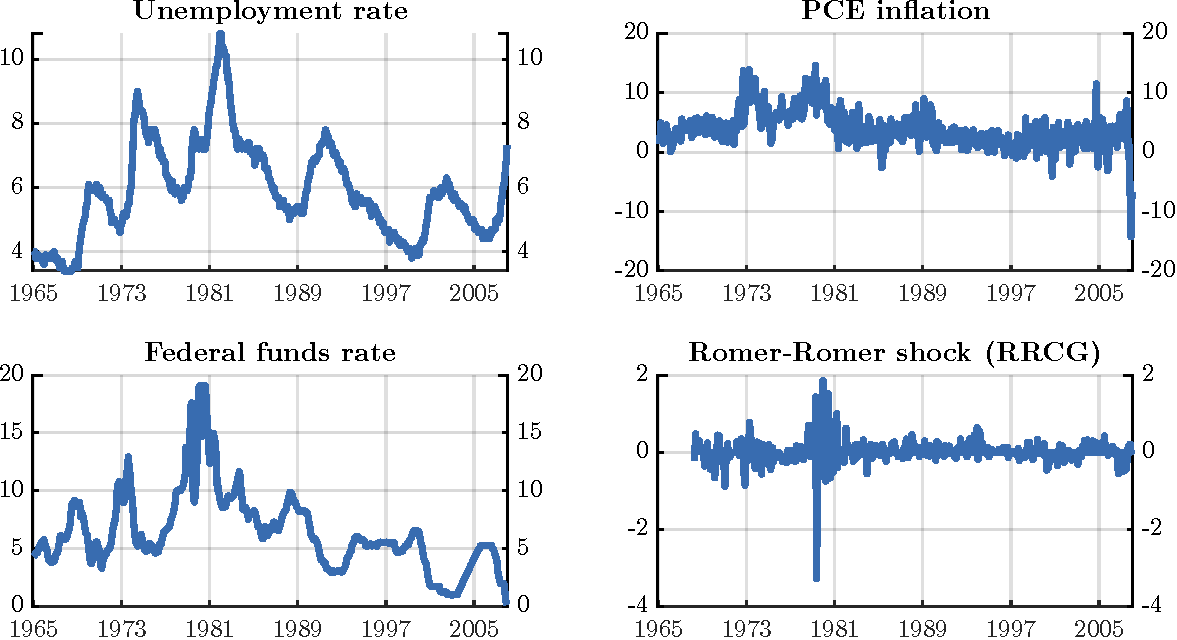
\includegraphics[width=\textwidth]{JT_Data_IV.pdf}
\end{minipage}
\end{frame}

%------------------------------------------

\begin{frame}
{\textbf{Identification: LP-OLS vs.\ LP-IV}}
\begin{itemize}
\item \textbf{LP-OLS} \ The Romer-Romer narrative shock $s_t$ is assumed exogenous and enters the regression directly as the treatment. No instrumentation is required\bigskip
\item \textbf{LP-IV} \ The federal funds rate $d_t$ is endogenous (the Fed responds to economic conditions). The RRCG narrative shock $z_t$ instruments $d_t$ via 2SLS at each horizon\bigskip\pause
\item \textbf{Both use long-difference LHS:}
\begin{equation*}
y^*_{t+h} \equiv y_{t+h} - y_{t-1}
\end{equation*}
Appropriate for persistent series; avoids level-stationarity issues
\end{itemize}
\end{frame}

%------------------------------------------

\begin{frame}[fragile]
{\textbf{Replication: LP-OLS (Example 5)}}
\begin{itemize}
\item CPI response to the Romer-Romer shock; LHS in long-difference form; 18-quarter horizon. \texttt{LPmodel} returns a struct \texttt{LP\_OLS} with fields \texttt{.IR}, \texttt{.INF}, \texttt{.SUP}
\par\smallskip
\begin{matlabcode}
% LP-OLS -- log CPI response to Romer-Romer shock (quarterly)
LPopt_OLS          = LPoption;
LPopt_OLS.nsteps   = 18;        % 18-quarter horizon
LPopt_OLS.longdiff = 1;         % LHS: lcpi_{t+h} - lcpi_{t-1}
LPopt_OLS.impact   = 1;         % unit shock
LPopt_OLS.pctg     = 95;
CTRL_OLS = [dlrgdp dlcpi dstir];
LP_OLS   = LPmodel(lcpi, rr_shock, CTRL_OLS, 4, 1, LPopt_OLS);
IR_OLS     = LP_OLS.IR;
INF95_OLS  = LP_OLS.INF;
SUP95_OLS  = LP_OLS.SUP;
\end{matlabcode}
\medskip
\item \colorbox{script!80}{\small\texttt{LPmodel}} signature: \colorbox{script!80}{\small\texttt{LPmodel(Y, S, CTRL, nlag, const, LPopt)}} --- \colorbox{script!80}{\small\texttt{S}} is the shock or instrument; lag order \colorbox{script!80}{\small\texttt{nlag}} applies to controls
\end{itemize}
\end{frame}

%------------------------------------------

\begin{frame}[fragile]
{\textbf{Replication: LP-IV (Example 6)}}
\begin{itemize}
\item Unemployment response to federal funds rate shock; RRCG narrative shock as instrument; 49-month horizon
\par\smallskip
\begin{matlabcode}
% LP-IV -- unemployment response to FFR shock (monthly)
LPopt_IV          = LPoption;
LPopt_IV.nsteps   = 49;        % 49-month horizon
LPopt_IV.longdiff = 1;         % LHS: urate_{t+h} - urate_{t-1}
LPopt_IV.impact   = 1;         % unit shock
LPopt_IV.pctg     = 95;
LPopt_IV.IV       = RRCGShock;
LPopt_IV.nlag_iv  = 6;         % lags of instrument
CTRL_IV = [urate infl ffr];
LP_IV   = LPmodel(urate, ffr, CTRL_IV, 6, 1, LPopt_IV);
IR_IV     = LP_IV.IR;
INF95_IV  = LP_IV.INF;
SUP95_IV  = LP_IV.SUP;
\end{matlabcode}
\medskip
\item \colorbox{script!80}{\small\texttt{LPopt.IV}} holds the \textbf{external instrument} (not the treatment); the endogenous treatment is the second argument to \colorbox{script!80}{\small\texttt{LPmodel}}
\end{itemize}
\end{frame}

%------------------------------------------

\begin{frame}
{\textbf{Results: Figures 5a and 6a}}
\begin{itemize}
\item LP-OLS: CPI falls by 2--4\% cumulatively after a contractionary shock. LP-IV: unemployment rises, with the response building over 12--24 months
\end{itemize}
\begin{figure}[h]
\centering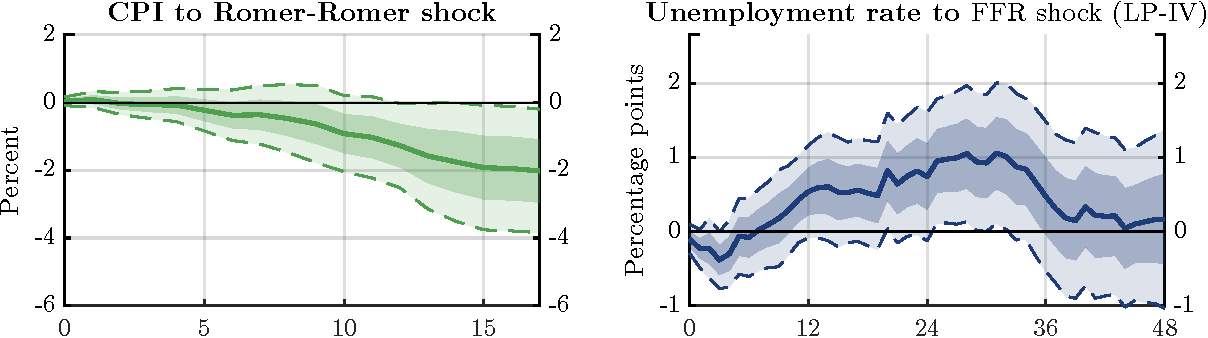
\includegraphics[width=.85\textwidth]{JT_Fig5a_6a.pdf}
\end{figure}
\end{frame}

%===============================
\appendix
\section{References}
%===============================

\begin{frame}
\color{title} \centering{\huge \textbf{Appendix}}
\end{frame}

%------------------------------------------

\begin{frame}[allowframebreaks]{References}
\scriptsize
\bibliographystyle{ecta}
\bibliography{BIBLIO.bib}
\end{frame}

\end{document}
